\chapter{Fundamentals}
	\par This chapter is dedicated to illustrate some fundamental knowledge in order to fully understand the work I have done while investigating specific applications. Some of them are technologies arised in last ten years, improving not only the efficiency but also the stability and portability of the standard development of mobile applications. \newline
	Generally Android mobile applications are client implementations for specific services. The scenario is therefore the classic client-server communication model where each client interacts with one or more server. \newline
	\par First of all client and server must establish a connection between them, hopefully a \textit{secure connection}. This is the first topis explained in this section. Client and server, that means mobile application and application server, agree to find a secure way to communicate each other. 
	\par Once the connection is established there are lots of ways in which an application can send information. This is the problem of the data serialization. Informations can be represented using different Interface Description Languages (IDL). Starting from the classic JSON or XML format, passing through binary. Each representation has advantages and disadvantages. In particular there is a section dealing with an IDL that is widely used in mobile application, that is \textit{Protocol Buffer}.
	\par After having described the interation of a standard mobile application, there is a section explaining the concept of RPC, and in particular the recent developed \textit{gRPC} framework. As I said most of the mobile applications reflect the client-server paradigm. It is modern framework able to delegate some procedure in the client to the server, improving performance and portability of the application service.
	\par Finally the last section of this chapter deals with a new network procol called \textit{QUIC}, a modern evolution of the HTTP/2 protocol used by most of the recent applications.
		
	\section{HTTPS: HTTP over TLS}
		\par As stated in the online documentation for Android Developers~\cite{android_dev_tips} it is a good practice to protect applications data using the \textbf{Transport Layer Security (TLS)} along with the standard HTTP protocol. \newline
		TLS is a protocol designed to provide communications security over a computer network.  
		It provides \textit{confidentiality}, \textit{authentication} and \textit{integrity} meaning that: data is encrypted for third parties, ensure that both parties actually are who they pretend to be, ensure that data is not modified in the transit.
		\par A server (or web application) that wants to use TLS must have installed an \textbf{SSL certificate} on the machine. This certificate is released by a \textbf{Certificate Authority (CA)} for a specific domain, and contains important informations on the owner of that domain together with the public key of the server.  
		\par Every time a client wants to establish a connection with a server using TLS, the TLS Handshake procedure is issued.	
		\par There are also some mitigations Android mobile application developer can use in order to limitate authority checks
		
		\subsection{SSL/TLS Handshake}
			\par During the TLS handshake both mobile application and server exchange informations to set up a bidirectional encrypted connection. For this reason TLS version (1.0, 1.2, 1.3, etc) and cryptographic suite are agreed. Moreover the client verifies the authenticity of the server basing on its certificate. Finally both the endpoints will generate session keys to encrypt and decrypt the messages they will exchange each other. Once data are encrypted, they are signed with a Message Authentication Code (MAC), so that the receiver can verify the integrity of the data sent over the network.
			\begin{figure}[ht]
				\centering
				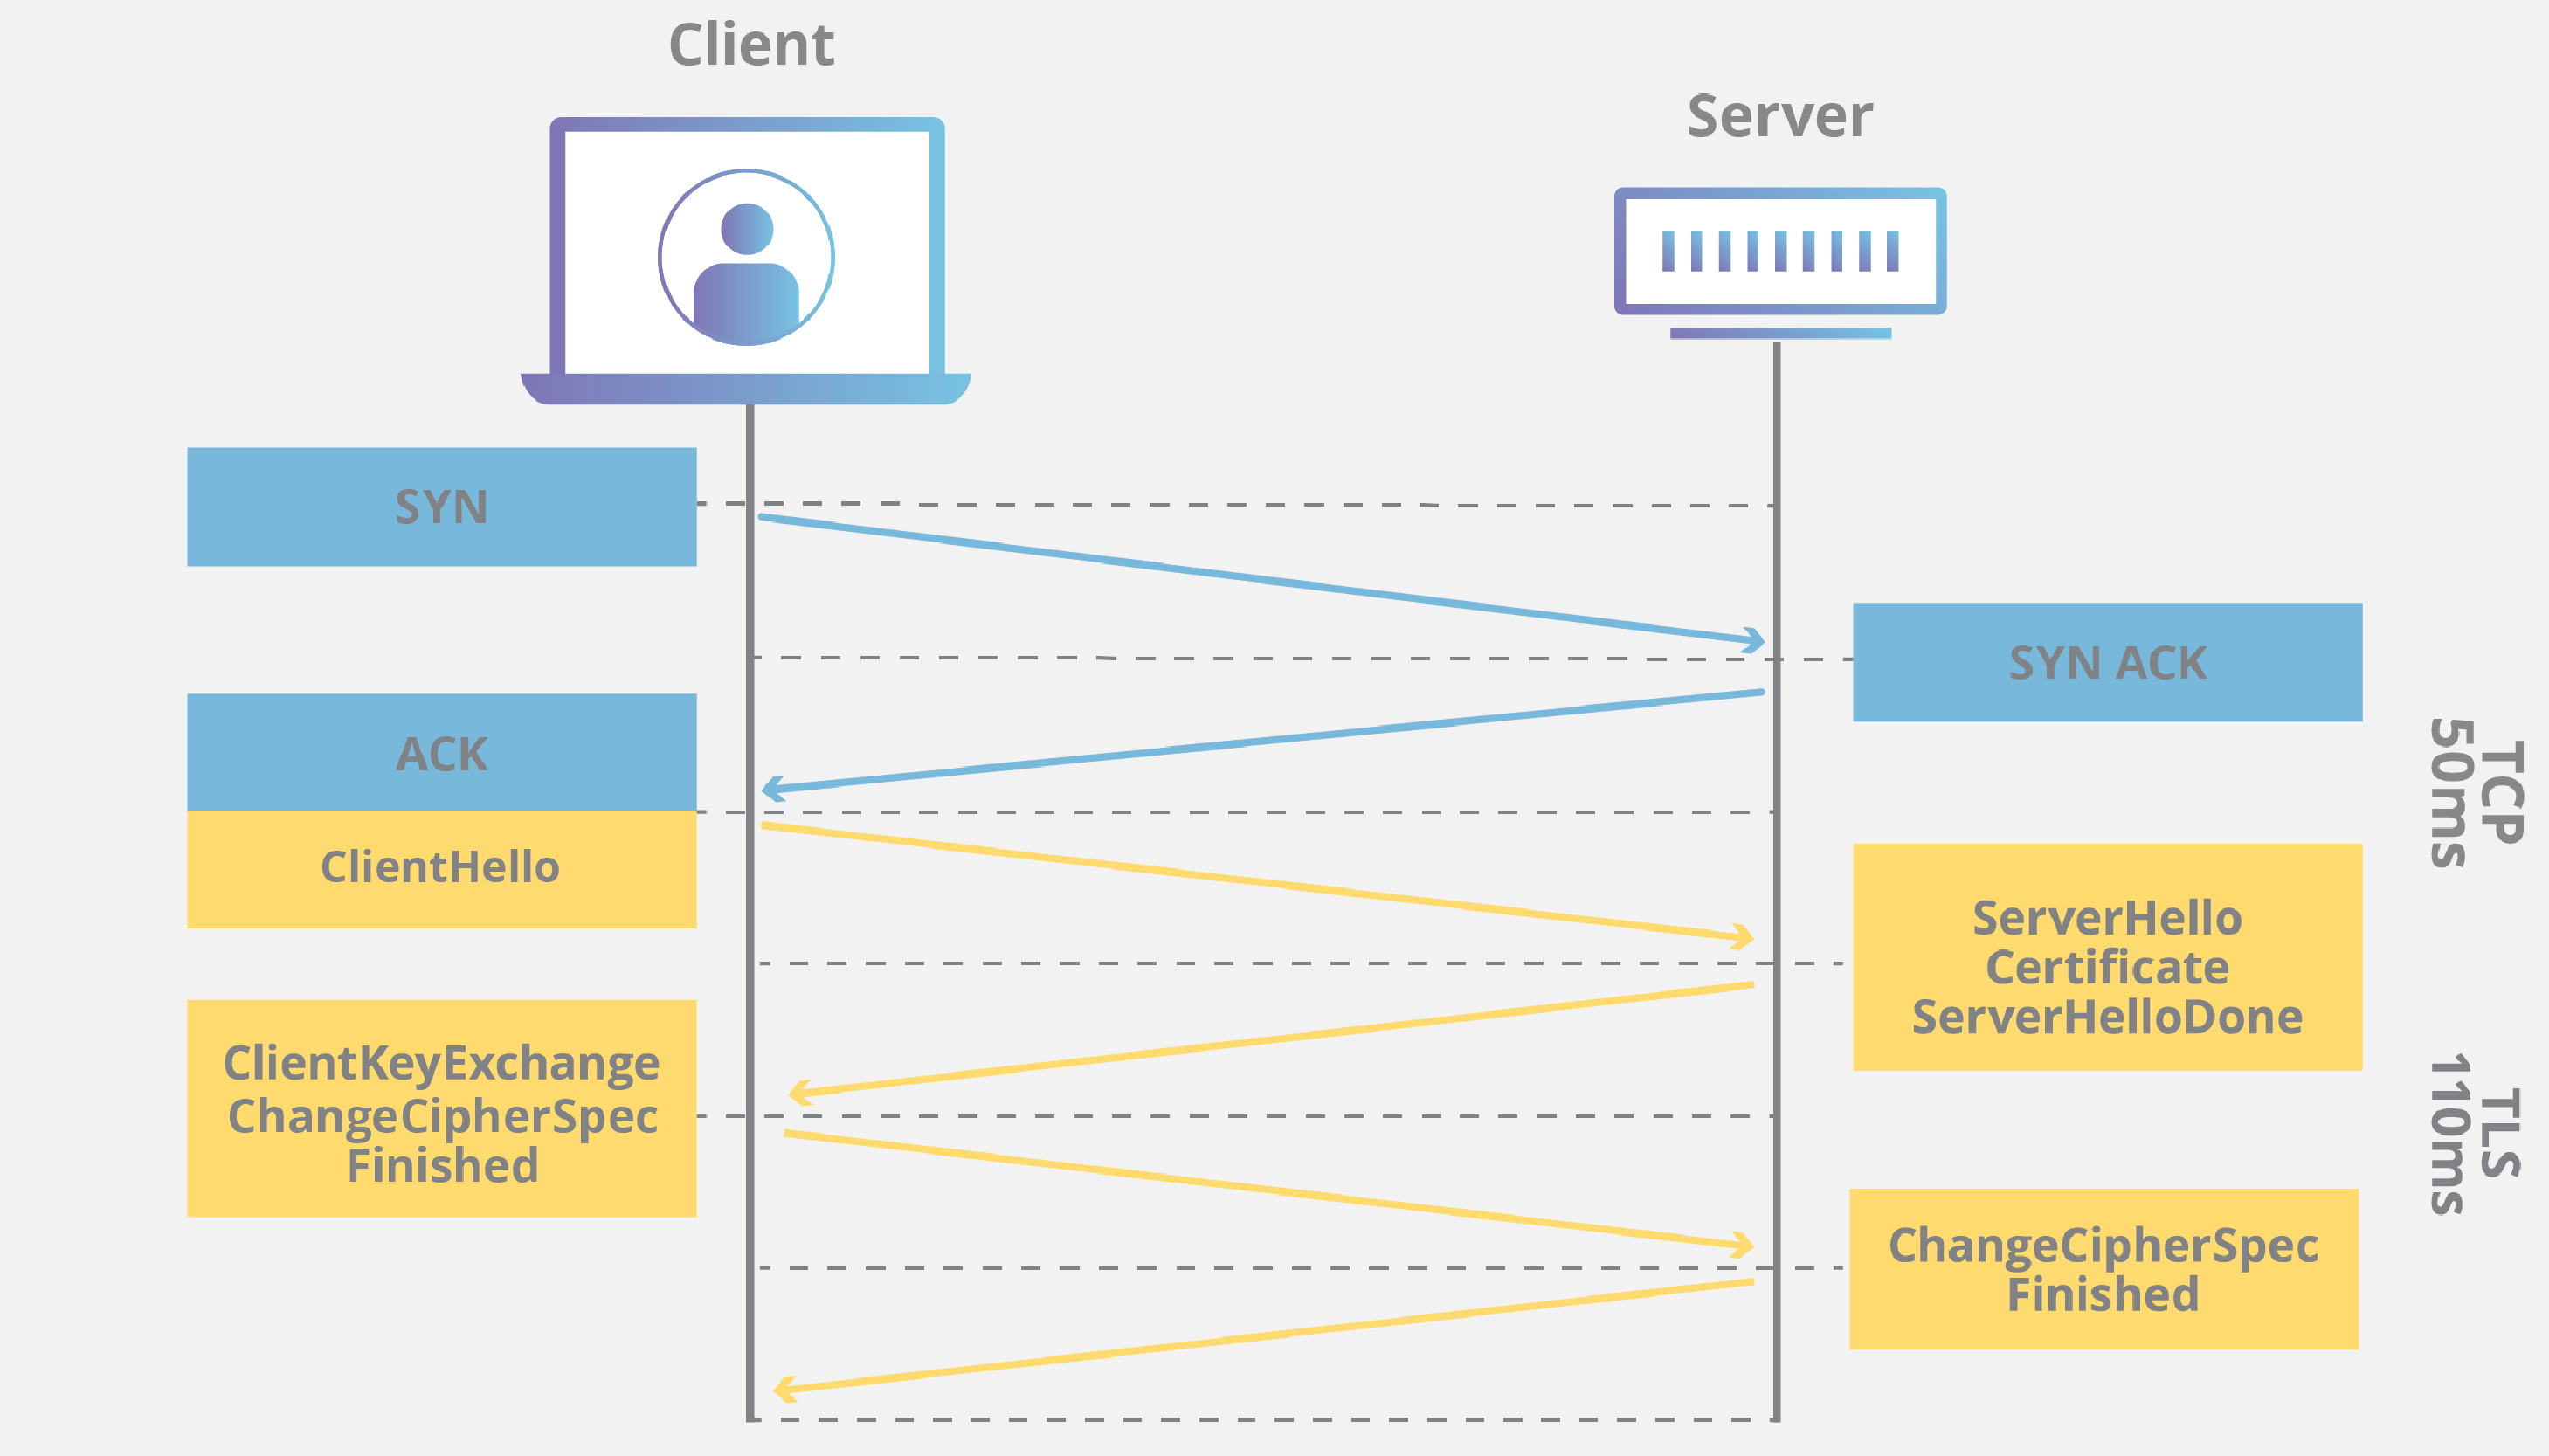
\includegraphics[width=0.8\textwidth]{images/tcp-tls-handshake.png}
				\caption{TCP Handshake and TLS Handshake communication flow needed to set up a secure connection. \cite{image_tcp_tls_handshake}}
				\label{fig:tcp_tls_handshake}
			\end{figure}
			\par From the performance point of view, the whole process of the TLS handshake needs both the endpoints to communicate before the data are actually transmitted over the network. In particular in the TLS versions < 1.3, two round trip time are needed to set up the whole connection \textit{(110ms)}. This amount of time added to the standard TCP three-way-handshake \textit{(50ms)} to establish the session between client and server, results in average in less then \textit{0.2 seconds} spent only to set up a secure connection without actually sending any application data yet. 
			\newline
 			As I said TLS makes possible to exchange information over a non-secure channel by providing confidentiality, authentication and integrity.  
			
		\subsection{Certificate Verification}
		\label{subsec:certificate_verification}
			\par A procedure I would like to stress is the certificate validation routine that happens at the really start of every TLS handshake. At the moment the client wants to establish a connection with the server, it needs the certificate to check the server is the actual endpoint the client want to talk with. The first thing the client does is to check that the certificate showed by the server is not expired, and that the server domain name matches with the one reported in the certificate. The next step performed by the client is to verify that the certificate has been signed by the certificate authority that authorized it. This procedure is done by verifying that the issuer's CA name matches the owner's CA name at the above level, and using the owner's CA signature and public key to verify the certificate is properly signed. The process is repeated until a CA trusted by the client is met, usually a root CA.
			\begin{figure}[ht]
				\centering
				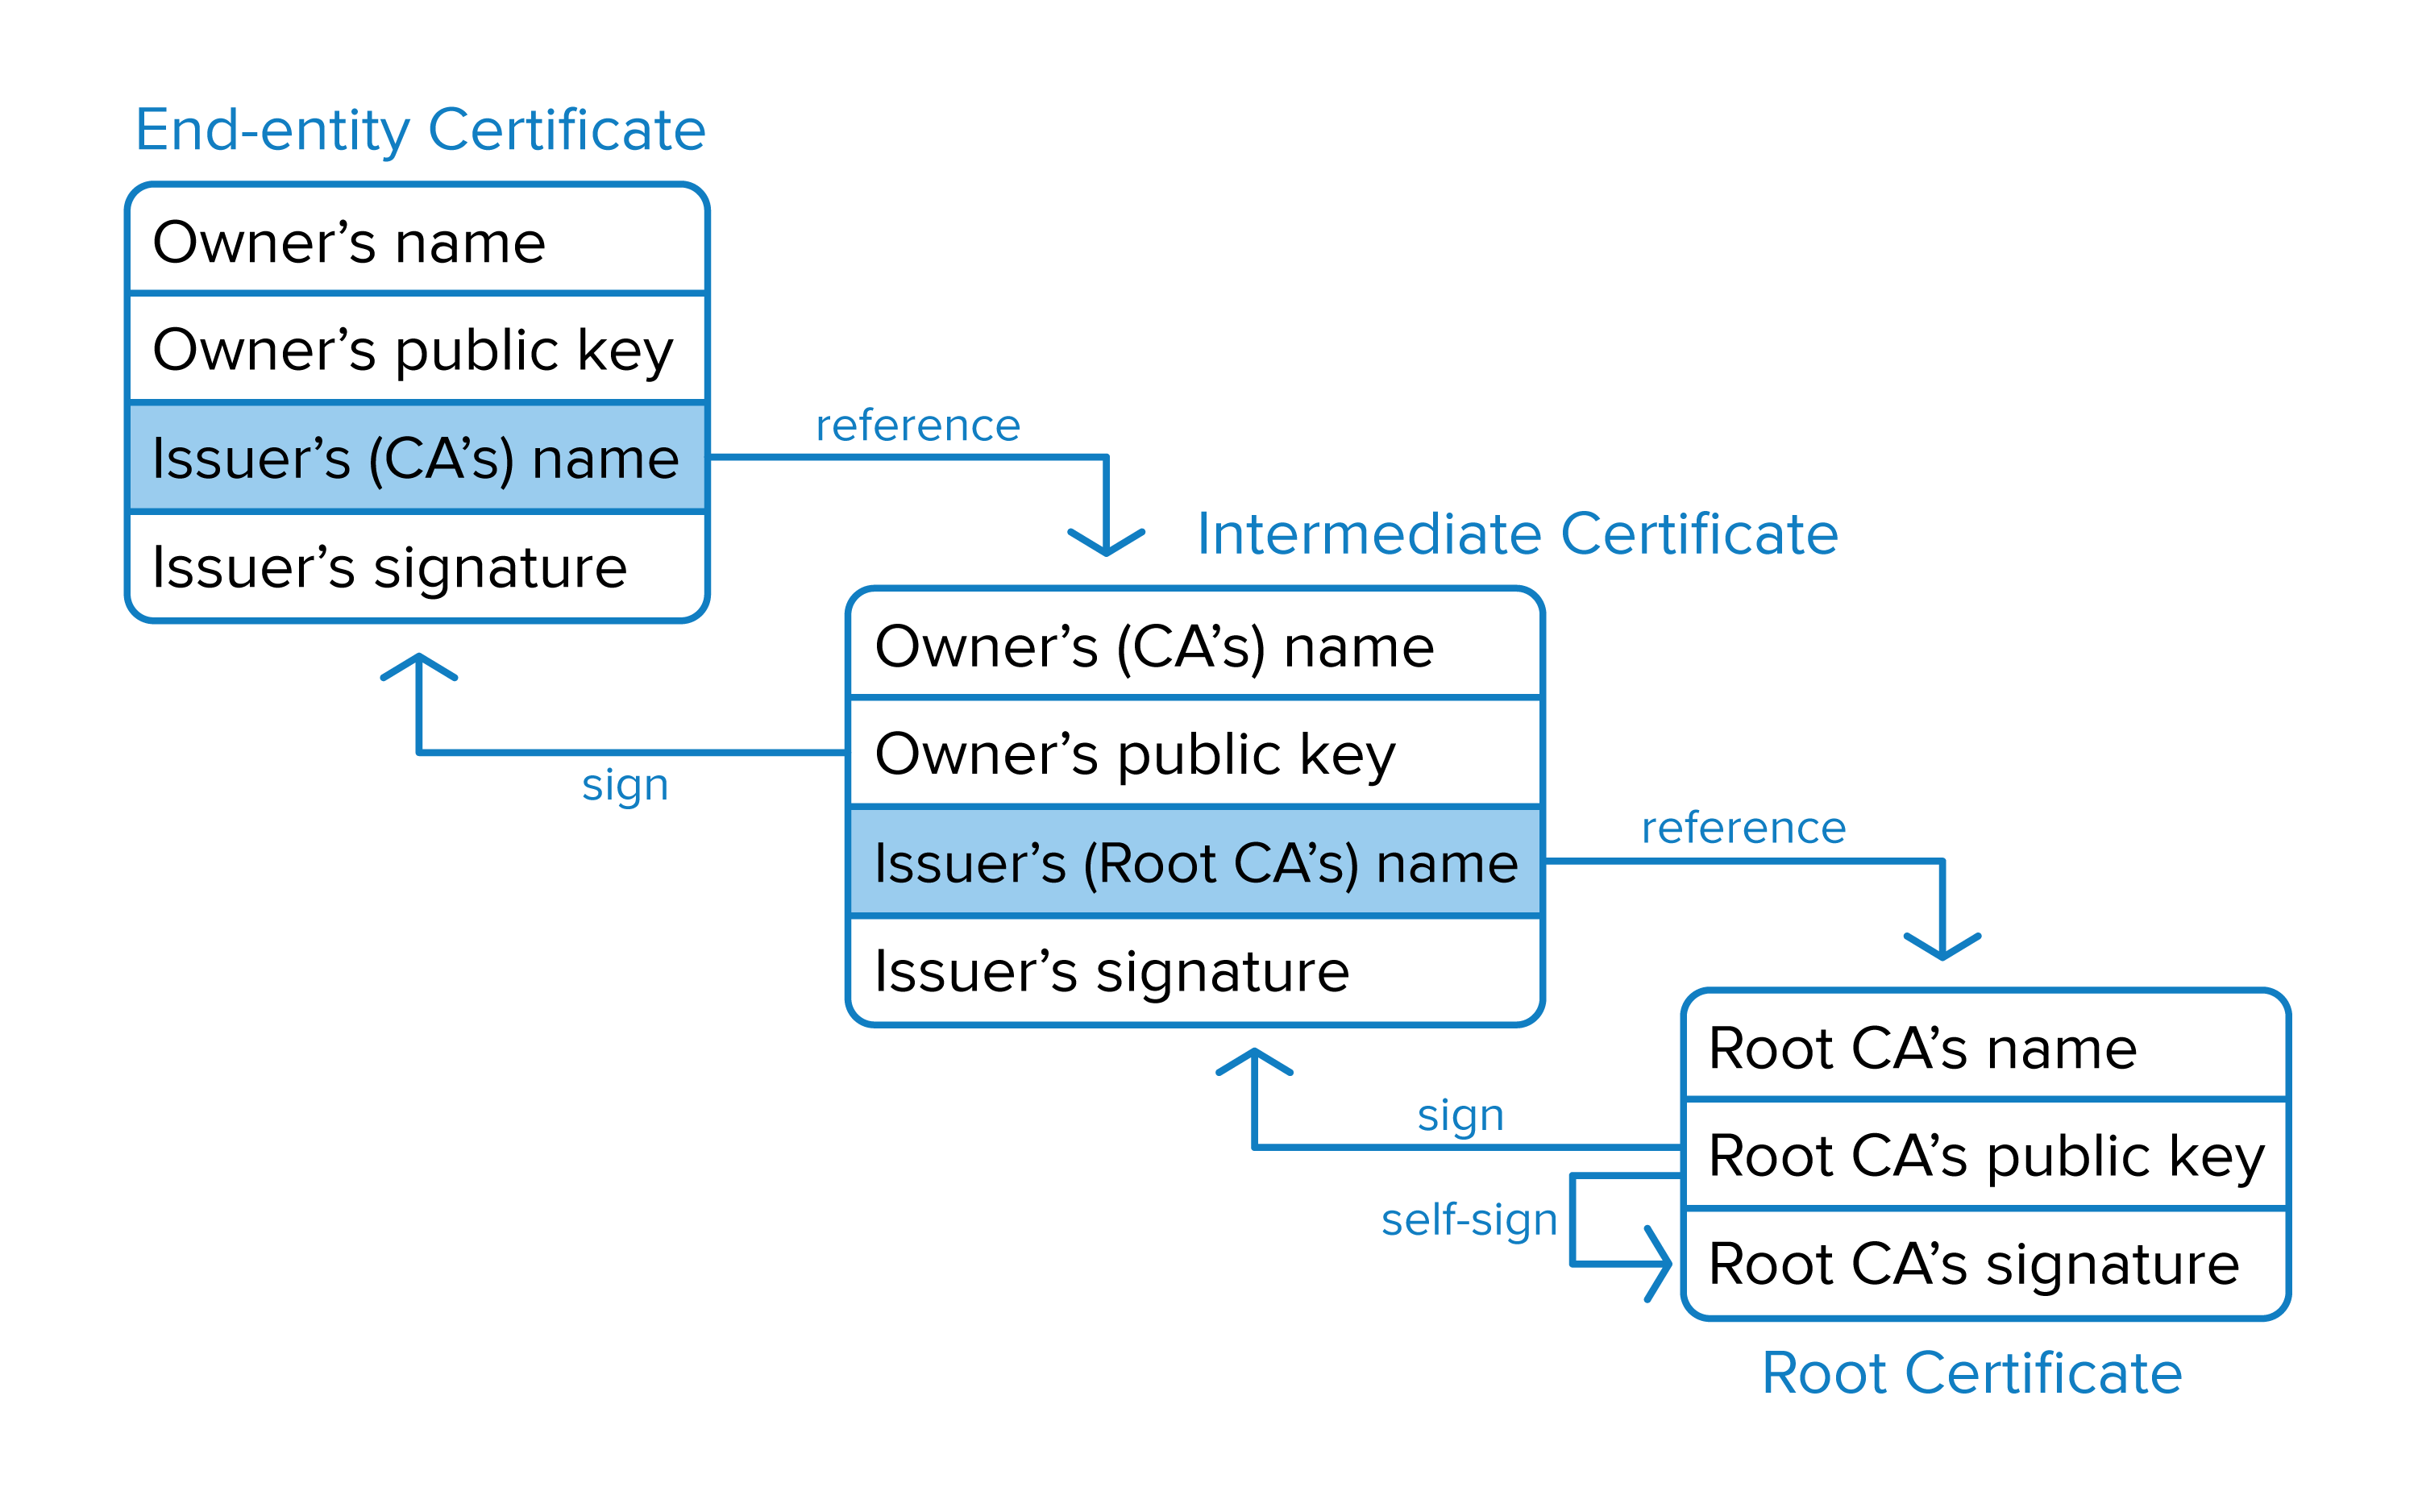
\includegraphics[width=0.8\textwidth]{images/tls-certificate-verification.png}
				\caption{TLS Certificate verification chain. \cite{image_tls_certificate_verification}}
				\label{fig:tls_certificate_verification}
			\end{figure}
			\par Usually certificates are bought by companies that wants to implement a secure connection with their clients. In this way the certificate obtained by the server is inserted in the tree of certificates, and every client can verify its authenticity. Note also that every machine can generate a self-signed certificate. What is indeed important is checking if the server certificate is linkable to a trusted Certificate Authority. \newline
			\par The Android operative system handles by itself a list of trusted certificates. These certificates belong to two categories: system certificates and user certificates. \newline
			\textit{System certificates} are used by default to verify all other certificates. So if we are using an application trying to connect to an application service, if the certificate obtained by the web service is traceable to one certificate already present in the system store, then the certificate is accepted and the connection is established. Notice that since the release of Android 7 Nougat, it is impossible to install any CA at system level without having root privileges on the device. \newline
			On the other way \textit{user certificates} are installable even at user level, and are used to verify certificates when directly expressed by the application.
			
		\subsection{Man-in-The-Middle}
		\label{subsec:mitm}
			\par \textbf{Man-In-The-Middle (MITM)} is an attack able to disrupt the security properties delivered by the TLS protocol. As the name suggests the attacker positions himself between the server and the client. The attacker acts like a proxy server intercepting every connection incoming from the client, pretending to be the real server, and forwarding them to the real server, pretending to be the real client. 
			\par On one side, at the moment of the TLS handshake, the client verifies the identity of the server, so the attacker needs to reproduce the handshake with the client in order to let it trust the attacker. As described in the last section, the authenticity check is performed through the exhibition of the server certificate. In this case the client needs to trust the certificate of the attacker. After having checked the identity of the server, the TLS handshake can continue following the standard procedure: client and attacker agree on a pre-master shared key and the encrypted communication will take place.
			\par On the other side the attacker needs to act as the real client for the server, so that every connection intercepted will be redirected to the server, and every response obtained will be delivered to the client. This is made possible by starting a new connection between attacker and server. The attacker will authenticate the server by checking its certificate and completing the standard TLS handshake with it. \newline
			At this point the attacker has performed two different TLS handshakes, one with the client faking to be the server, and one with the server faking to be the client. The man in the middle is now able to read messages sent or received from the client and forward or deliver them to the server. \newline
			\par A man-in-the-middle attack is what made possible the analysis of the communication protocol of every application I investigated. After having \textit{placed} ourselves inbetween client and server we will be able to understand what exactly is the protocol adopted by an android application and analyze each message looking for a possible leak detection of users personal data. For more specifics on how I performed a MitM attack for my case studies, read the chapter \textit{Testing Environments}, sections \textit{HttpToolkit}[Section \ref{sec:http_toolkit}] and \textit{BurpSuite}[Section \ref{sec:burp_suite}].
			
		\subsection{SSL Certificate Pinning}
			\par If the MitM attack results in the loss of authenticity in an HTTPS communication, the \textbf{SSL Certificate Pinning} is an hardening process that can be adopted in order to deliver an additional layer of security to the software. Pinning certificates or public keys is a countermeasure that allow web servers to control the risk of man-in-the-middle attacks or CA compromise. 
			\par The whole process of certificate verification described in the previous section is skipped, the application will indeed only validate certificates or public keys that are \textit{pinned} to the application. A MitM attacker will not be able to intercept messages anymore. The connection will be blocked right in the middle of client's and attacker's TLS handshake. The application implementing a certificate pinning method in fact will not trust anymore the attacker's certificate, and the connection will be dropped by the attacker's proxy.
			\par There are two ways of implementing this hardening technique. The first one is by \textit{preloading} the public key or certificate in the client at development time, so that every fake server trying to connect to the client is rejected during the TLS handshake phase. The second one happens at runtime by installing the \textit{pin} in the client once upon the connection is established by using the HTTP Public Key Pinning (HPKP) header, indicating the public key and the max age of validity for that specific pin. This second approach has been adopted by Chrome and Firefox for their browsers, but after some years new security issues has been discovered about it. Indeed in case of bad implementation (for example a pin of an incorrect public key) could bring to denial of service, but even in case of compromised server the consequences can be devastating for a longer time if HPKP is implemented, a bad pin might be established from an attacker that had the control of the server (HPKP Suicide~\cite{HPKP_suicide}). For this reason the public key pinning is now highly discouraged for web browsers. \newline
			\par In Android application SSL certificate pinning is a solution still able to protect from MitM attacks. The implementation is generally done by pinning a specific certificate inside the application logic at development time. There are multiple ways to implement a certificate pinning in Android as explained in \cite{android_ssl_pinning}. Among them two approaches can be identified: 
			\begin{enumerate}
				\item basing on \textit{Network Security Configuration}: A pretty simple certificate pinning implementation made possible by specifying a \textit{<domain-config> tag} in the network security configuration file present in the application. A \textit{pin-set} of \textit{pin} can be specified for the whole application.
				\item basing on the \textit{network library}: Many different network libraries exist for Android application (i.e. \textit{OkHttp}, \textit{Retrofit}, \textit{Volley}, and so on). Each one of them provide methods to skip the standard certificate validation procedure and implement the certificate pinning procedure.
			\end{enumerate}
			
		\subsection{Certificate Transparency}
		\label{subsec:certification_transparency}
			\par \textbf{Certificate Transparency} (CT) is a security standard adopted by browsers for monitoring and logging discrepancies in the certificate verification procedure. The whole system is manteined by a set of certificate logs handled by Certification Authorities and many browsers. These logs assume the form of \textit{Merkle trees} (also noticed as \textit{hash tree}), they are publicly verifiable, in append-only mode. The goal of this standard is to keep track of all valid certificates ever issued for a specific domain. \newline
			\par	This is the scenario: a domain owner implementing a web service requests a new certificate from a CA. Before releasing the new certificate, it submits the \textit{hash digest} of that certificate to one or more certificate logs, receiving a \textit{Signed Certificate Timestamp (SCT)} signed by the log provider. Once signed, the CA can now send back the certificate with embedded the SCT to the domain owner asking for the certificate. Every HTTPS connection to that web service will be served using that certificate. When a user wants to use the web service, browsers or mobile apps will query the trusted certificate log to find a record matching with the SCT of the certificate received by the web service. \newline
			\par In Android operative system, an example of application implementing the Certification Transparency mechanism is the Chrome browser. As we said above (see Certificate Verification [Section \ref{subsec:certificate_verification}]) Android certificates can be placed at system level or user level. Every application will use by default the system store to verify others certificates, and so does Chrome, if not specified differently. This application will choose whether to use the Certificate Transparency or not, basing on which store the certificate root is installed. When a certificate showed by any web service it is checked, if the root certificate met is present in the system certificates store then Chrome decides to also verify the Certificate Transparency requirement. On the other way if we are testing a web service showing a certificate that is inside the user certificates store, then the Certificate Transparency procedure is not applied.\newline 
			
	\section{Protocol Buffers}
	\label{sec:protocol_buffer}
		\par \textbf{Protocol Buffers}\cite{protocol_buffer}, also known as ProtoBuffers, are a language-neutral, platform-neutral extensible mechanism for serializing structured data. The development of this new mechanism started in the early 2001 from Google for private purposes. Then in the 2008 was publicly released as open-source data format. The design goal while developing Protocol Buffers was to provide a data serialization universal and faster then the standard XML. Nowadays it is widely used when an internaction between different architectures client-server is needed, that is the case for most of the Android application.
		\par The messages exchanged are data structures described in a proto definition file \textit{.proto}. After having compiled those definitions through \textit{protoc} they can be imported in any project written in the most used programming languages. Protobuf version 2.0 was providing a code generator compatible with \textit{C++}, \textit{Java}, \textit{C\#} and \textit{Python}. The version 3.0 extended the programming language compatibility also to \textit{Go}, \textit{Ruby}, \textit{Objective-C}. Other languages are supported through third-party implementations (\textit{C},\textit{JavaScript}, \textit{Perl}, \textit{PHP}, \textit{Scala}). 
		\par To give an idea on how the mechanism works, let's say a client-server application would like to serialize data about a \textit{Person}. In order to let both endpoint to know about the data structure \textit{Person}, both of them require to integrate in their project that data structure. The definition of \textit{Person} is done in a \textit{.proto} file:
\begin{lstlisting}
message Person {
	optional string name = 1;
	optional string email = 2;
	optional string phone = 3;
}
\end{lstlisting}	
		The proto file has to be done only once, and it is independent from the platform we will be using. To import the definition of the above \textit{Person} data structure in our project we need to run the \textit{protoc} compiler obtaining the ready-to-use structure. \newline
		\par Since the native language for Android application is Java, running \textit{protoc} we are interested in the \textit{.java} classes generated. For each message type defined in the \textit{.proto} file will result a couple of \textit{.java} files: one will contain the definition of the object itself, the other one is the Builder for that specific object type. The first one will be provided of the standard accessor's methods (in our case \textit{hasName()}, \textit{getName()}, and so on for each field), while the second one will have both getters and setters methods (\textit{getName()}, \textit{setName()}, and so on for each field). At this point it is needed to import those definitions in \textit{.java} classes thanks to the Protocol Buffer API provided by the mechanism itself. This is a picture summarizing the whole procedure:\newline
		\begin{figure}[ht]
				\centering
				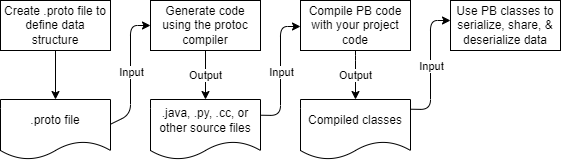
\includegraphics[width=0.9\textwidth]{images/protobuffer.png}
				\caption{Procol Buffer workflow \cite{protocol_buffer}}
		\end{figure}
		\par Each object already instantiated is immutable, it can only be modified through its respective Builder methods at the moment of its building. The procedure to instantiate a new \textit{Person} object in the application is respectively: 
		\begin{enumerate}
			\item Contruct a builder for the object. 
			\item Set any field to any acceptable value.
			\item Call the builder's \textit{build()} method.
		\end{enumerate}
		\par In particular the step 2 is made possible through the mehods provided automatically in those \textit{.java} files. Each one of them will modify the structure created at step 1, and it will return a new \textit{Builder} object, such that it can be repeatedly modified and at the end instantiated through the \textit{build()} method. \newline
		\par The above defined \textit{Person} class, it is just an example. The Protocol Buffer mechanism is able to provide a platform-independant really complex classes with repeated fields, nested classes, constant values or even rpc services to define. At the same time the use of Protocol Buffer let the developer save time  when developing the data structures. Indeed the \textit{.proto} definition has to be done only once, and it is valid for every kind of platform that would use that type of structure.

	\section{gRPC}
		\par \textbf{gRPC} \cite{grpc} is a cross-platform \textit{Remote Procedure Call} (RPC) framework. The mechanism was initially created by Google for private purposes, but in 2016 it was publicly released as open-source. As a remote procedure call framework, it let the developer to define in an application some methods that will actually run on a different machine from the one running the application. Generally the idea behind any RPC system is to define a \textit{service} able to execute a specific method in order to call it remotely from any another application.
		\begin{figure}[ht]
			\centering
			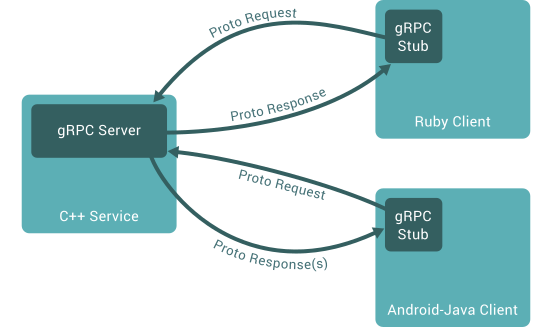
\includegraphics[width=0.7\textwidth]{images/grpc.png}
			\caption{gRPC workflow \cite{grpc}}
		\end{figure}		
		\par What makes gRPC so powerful is the fact it is based on \textit{HTTP/2} protocol for the transport layer, and uses \textit{Protocol Buffers} (described in Section \ref{sec:protocol_buffer}) as its Interface Description Language (IDL). The combination of these two mechanism let the gRPC system to provide an easy access and platform independant solution for the implementation of a RPC system. \newline
		In a gRPC system, as any other RPC system, we can differentiate between \textit{gRPC Server} and \textit{gRPC Stub}, the part of the client implementing the gRPC framework. On the server side, the server implements the interface for the specific method it is able to execute, and handles the incoming client calls. On the client side, the gRPC Stub provides the same method as defined by the server. What really happens in the moment in which the client invoke the method is that:
		\begin{enumerate}
			\item The gRPC Stub serializes the parameters passed to the method using the Protocol Buffer mechanism. Then sends over an HTTP/2 connection the method request together with the serialized data.
			\item The gRPC Server accepts the incoming request from the client and deserializes the data using the Protocol Buffer mechanism.
			\item The gRPC Server will execute the method specified by the client.
			\item Once the result is available, the gRPC Server sends over the HTTP/2 connection the response containing the return value for that specific method, serialized with the Protocol Buffer mechanism.
			\item The gRPC Client deserializes the return value using the Protocol Buffer mechanism.
		\end{enumerate}
		\par Even if different IDLs can be specified while defining the gRPC service, JSON for example, by default the gRPC framework uses Protocol Buffers. Moreover the framework provides features like \textit{authentication} (through TLS or token-based authentication) and \textit{bidirectional streaming}.
		
	\newpage
	\section{QUIC}
		\par \textbf{QUIC} is a general-purpose transport layer network protocol designed by Google. It was publicly announced in 2013 and after some years under the experimental state, in the recent 2021 became a standard as defined from the Internet Engineering Task Force (IETF) in \textit{RFC 9000} \cite{rfc9000}.\newline
		\par The main goal of QUIC is to improve the performance of the connection-oriented web applications, that for years have been run basing on TCP as transport layer network protocol. QUIC establishes a number of multiplexed connections using UDP instead, allowing multiple streams of data to reach different endpoints independently. The same concept is possible in HTTP/2 with multiplexed connections, but what really suffers this last one is the the head-of-line-blocking delays related to the connection-oriented TCP which it relies on. \newline
		\par Briefly the \textit{Head-of-Line blocking} (HOL blocking) is an issued generally affecting every packet that need to pass through a line. If the First-In-First-Out (FIFO) method is used, the longer the packet has arrived in the queue, the higher is the priority it has to be sent over the line. With the release of HTTP/2, this issue was partially resolved through the multiplexing of multiple connection, letting multiple HTTP requests running together but still an implementation over a single TCP connection. If one packet is being lost in the transmission than the whole connection will be waiting for the retransmission of that single packet. Now in the case of a client with few connections towards a bunch of server is waiting time is neglactable, but modern Android applications are implementing different services at the same application, using both standard HTTPS requests and gRPCs with an high number of structures to serialize through Protocol Buffer towards hundreds of endpoints. In case of a packet retransmittion the performance loss will be evident.
		\par QUIC protocol addresses this issue by relying on \textit{UDP} as transport layer protocol. UDP is a connectionless transport layer protocol without any implementation of packet orderding and retransmission, indeed every packet is forwarded to the endpoint individually, without any risk of HOL blocking problem. At the same time UDP does not provide any guarantee on the packets delivery making the whole connection unreliable. All  these checks are in fact implemented in QUIC on top of UDP, while still taking advantage of the performances achieved by UDP. Every additional connection feature, like TLS encryption, is done in the same way on top of UDP. \newline
		\par The second goal of QUIC is to improve the connection latency between the two endpoints. Using UDP as transport layer protocol the TCP overhead needed for the connection management is already cutted off. Most of the applications will demand for TLS encryption requiring its own handshake, that would be summed up to the TCP three way handshake if using the HTTP/2 protocol. With QUIC there is no redundancy in those handshake phases. It is done only once in QUIC as showed below:
		\newline
		\begin{figure}[ht]
			\centering
			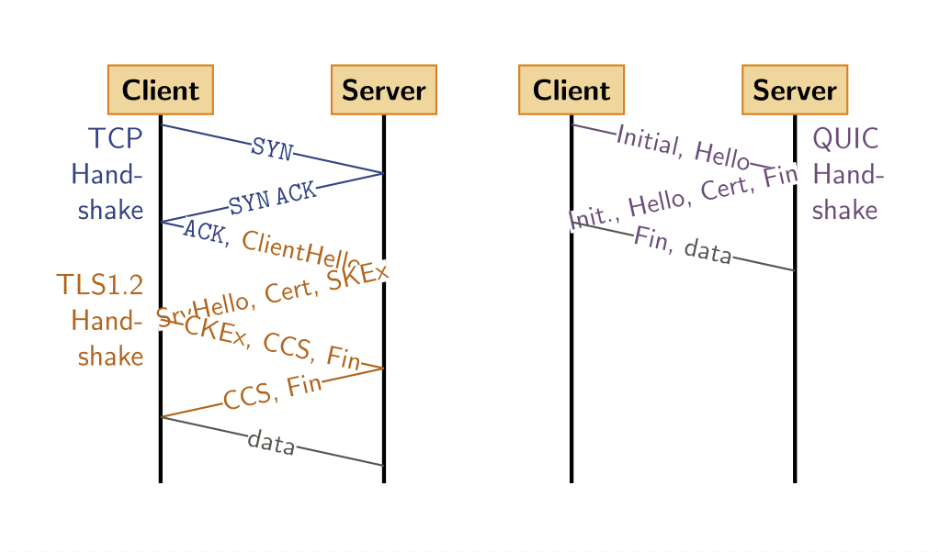
\includegraphics[width=0.8\textwidth]{images/quic_handshake.png}
			\caption{Comparison between TCP+HTTPS and QUIC handshakes}
		\end{figure}	
		\par Moreover, as said above, UDP does not handle loss recovery, meaning that QUIC is also resposible for each separated controlled flow. Others improvement in terms of overall latency are adopted, for example packets are individually encrypted, so that can not result in a waiting for partial packet.\newline
		\par Another property of QUIC is the ability to mantain its performance during network-switch events that frequently happens in mobile devices, like the connection transition between WiFi hotspot and mobile network. In HTTP/2, based on TCP, every connection is timed-out one by one and then re-established on the new network, while in QUIC at every connection is assigned an identifier that is kept even if the source ip address changes.
		\par Lastly, QUIC is completely handled at application level. There are numerous libraries available in order to implement this protocol in an application: \textit{Cronet} developed by Google, \textit{sn2-quic} developed by Amazon Web Services, \textit{proxygen} by Facebook and so on.\newline
		For a practical example see the application case Google Maps in Section \ref{sec:google_maps}.
	
		
		\subsection{HTTP/3}
			\par In June 2022 the IETF published \textbf{HTTP/3} as the major version of the \textit{HyperText Transfer Protocol} in \textit{RFC 9114}\cite{rfc9114}. Unlike the earlier versions of HTTP 1.1 and 2.0 based on TCP, HTTP/3 relies on QUIC, based on UDP. \newline
			\par HTTP/3 uses the same semantics of the previous versions (request methods, status codes, message fields) but it differs in the way it mantains the connection session. Most of the changes in HTTP/3 are in the way the protocol interfaces with the underlaying transport layer. The new version of HTTP results in lower latencies and higher performance in real-world usage, mostly due to the adoption of QUIC. 
